\documentclass{report}[12pt]

\addtolength{\oddsidemargin}{-.875in}
\addtolength{\evensidemargin}{-.875in}
\addtolength{\textwidth}{1.75in}
\addtolength{\topmargin}{-.875in}
\addtolength{\textheight}{1.75in}

\usepackage[latin1]{inputenc} % un package
\usepackage[T1]{fontenc}
\usepackage[francais]{babel}

\usepackage{amsthm}
\usepackage{amsmath}
\usepackage{amssymb}
\usepackage{mathrsfs}
\usepackage{graphicx}
\usepackage{wrapfig}
\usepackage{floatrow}
\usepackage{enumitem}
\usepackage[all]{xy}


\newcommand\tab[1][0.5cm]{\hspace*{#1}}

\newtheoremstyle{break}
  {20pt}% measure of space to leave above the theorem. E.g.: 3pt
  {20pt}% measure of space to leavebelow the theorem. E.g.: 3pt
  {\itshape}% name of font to use in the body of the theorem
  {20pt}% measure of space to indent
  {\bfseries}% name of head font
  {}% punctuation between head and body
  {\newline}% space after theorem head; " " = normal interword space
  {}
\theoremstyle{break}
\newtheorem{lemma}{Lemma}[section]
\newtheorem{corollaire}{Corollary}[section]
\newtheorem{proposition}{Proposition}[section]
\newtheorem{theorem}{Theorem}[section]
\newtheorem{definition}{Definition}[section]
\newtheorem{example}{Example}[section]
\newtheorem{exo}{Exercice}[section]
\theoremstyle{plain}
\newtheorem{remark}{Remark}[section]

\title{Construction of a quasi-geodesic on a linear sphere by piece}
\author{Jean Chartier}
%\date{}
\begin{document}
\maketitle



In 1949, Alexandre Pogorelov proves the existence of a simple and closed quasi-geodesic on any convex polyhedron\footnote{We give in the appendix the proof that there does not always exist a straight quasi-geodesic on a convex polyhedron, that is to say if necessary, which crosses the vertices forming two equal angles.}. We propose to describe an algorithm allowing to build such a quasi-geodesic on any linear sphere by pieces, not necessarily convex. We first prove the existence of a quasi-geodesic of length less than a bound depending on a triangulation of the faces. This gives us an upper bound on the combinatorics of the quasi-geodesic (order of meeting of the vertices and edges) and allows us to draw up a list of the paths to be tested. 
\begin{definition}[Quasi-geodesic]
A quasi-geodesic on a piecewise linear surface $S$ is a continuous path $\gamma : I\longrightarrow \partial S$, where $I$ is an interval of $\mathbb{R}$, satisfying four conditions :
\begin{itemize}
\item{It is uniform rectilinear on the faces of $ S $ that it crosses.}
\item{It forms on the passage of an edge two angles equal to $\pi$.}
\item{It forms on the passage of a vertex of positive curvature two angles less than or equal to $\pi$.}
\item{IIt forms on the passage of a vertex of negative curvature two angles greater than or equal to $\pi$.}
\end{itemize}
\end{definition}

\textbf{Notation} : Given a linear sphere by piece $S$ of vertices $p_1,\dots,p_n$, we consider a triangulation $\{T_1,\dots,T_l\}$ which is based on the vertices and which be shellable\footnote{ref}, that is to say : $$\forall i=1\dots l, \bigcup_{k=1}^{k=i}T_k\simeq D^2 \text{ et }\bigcup_{k=1}^{k=l}T_k\simeq S^2$$
From now on, we can work from the metric of $T_k$ and their combinatorics within $S$. We denote by $a_1, \dots, a_m$ the edges of this triangulation (old and new edges combined), or else if necessary, $a_{ij}$ the edge which connects the vertices $p_i$ and $p_j$. We call \textit{hat} of vertex $p_i$, denoted by $\mathcal {C}_i$, the union of the triangles $T_k$ having $p_i$ for common vertex. We specify that $T_i$ and $T_{i+1}$ are not necessarily adjacent. We optionally rename the vertices of $P$ to have $p_0\in T_1$ et $p_n\in T_l$.

\begin{theorem}[Existence]
Let $S$ be a linear sphere by piece as above. There is a simple and closed quasi-geodesic $\gamma : S^1\longrightarrow \partial P$ whose length does not exceed $M=\sum_i L(a_i)$.
%$M=\epsilon + \underset {(a,b,c)\pm P}{min}\; \underset{t\in \mathbb{R}}{max}\; L\left( \partial P\cap \{(x,y,z)\in \mathbb{R}^3 | ax+by+cz=t\}\right)$.\\
We can also ask, even if it means dragging $\gamma$ in parallel along the edges it crosses, that a point of $S^1$ be sent to a vertex $p_{\star}$.
\end{theorem}
\begin{proof}
We start by describing a sweep of $ S $ by simple loops, bounded in length. We sweep $T_1$ (resp. $T_l$) by segments $\sigma_s^1$ (resp. $\sigma_s^l$), parallel to the side opposite to $p_0$ (resp. $p_n$). Then, for $i$ from $2$ to $l-1$ :
\begin{itemize}

\item{If $T_i$ shares a single side with $\bigcup_{k=1}^{k=i-1}T_k$, we sweep $T_i$ by segments $\sigma_s^i$ parallel to this side.}
\item{If $T_i$ shares two sides with $\bigcup_{k=1}^{k=i-1}T_k$, we sweep $T_i$ by segments $\sigma_s^i$ parallel to the third side.}

\end{itemize}
At each segment $\sigma_s^i$ so pulled through a certain $T_i$, we continuously associate (in $s$ then in $i$) the parameterization of a loop formed by the edge of the disc $\bigcup_{k=1}^{k=i-1}T_k$, deprived of its intersection with $T_i$ and linked to $\sigma_s^i$ by two portions of the edge of $T_i$ (see figure below). For $i=1$ (resp. $i=l$), rather we connect $\sigma_s^i$ to $p_0$ (resp. $p_n$) by two portions of the $T_i$'s boundary. We have thus constructed a sweep of $S$ by circles $\beta:S^2\longrightarrow P$ -- where $S^2$ is seen as the quotient of the cylinder $[0,1]\times S^1$ by the relation which identifies the circles $(0, S^1)$ and $(1,S^1)$ to two points -- which is of degree 1 and which satisfies:
\begin{itemize}
\item{Each fiber $\beta(s,.):S^1\longrightarrow P$ is a single broken line on the surface of $S$.}
\item{There is a sequence of values : $0<s_1<\dots<s_{l-1}<1$ such that $\beta([0,s_i]\times S^1)=\bigcup_{k=1}^{k=i}T_k$.}
\item{$\beta(0,.)$ is the constant loop in $p_0$ and $\beta(1,.)$ is the constant loop in $p_n$.}
\item{$\forall s\in]0,1[,\beta(s,.)$ is a polygon of length $l_s$ drawed on $S$, traveled at constant speed $c_s=l_t/2\pi$.}
\end{itemize}
\begin{figure}[h!]
		\begin{center}
			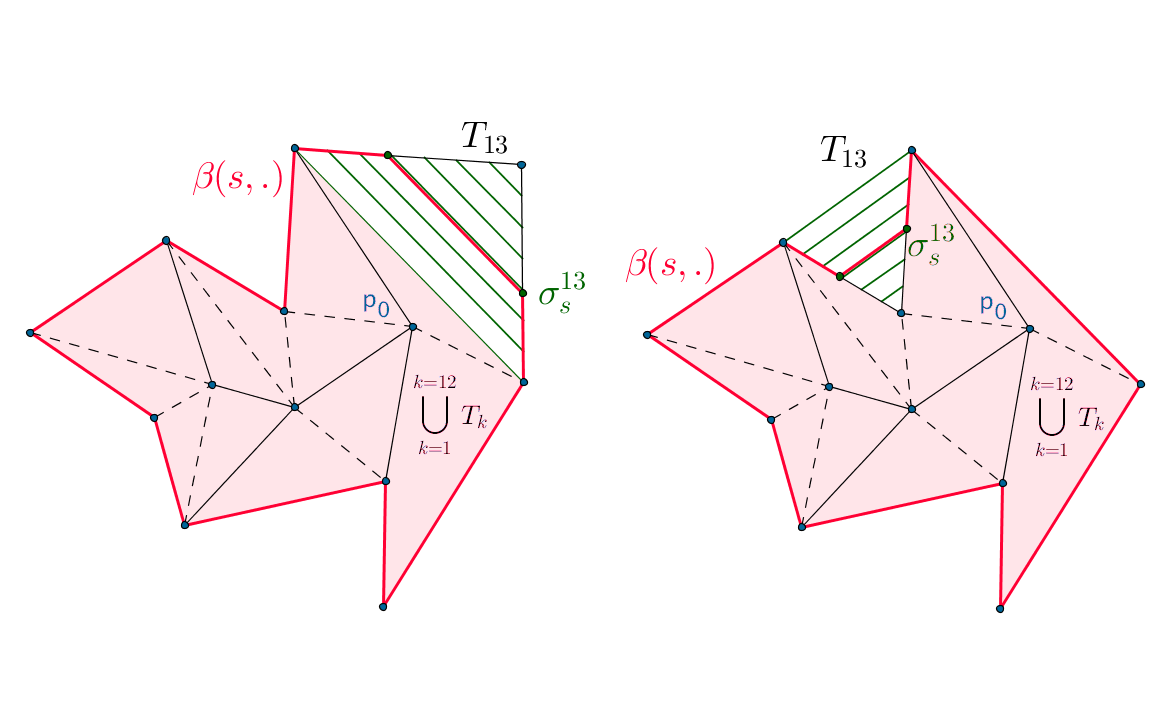
\includegraphics[scale=0.8]{epluchage2}  
		\end{center}
\end{figure}
Thus constructed, $\beta$ has no fiber $\beta(s,.)$ Whose length does not exceed $M$.\\ \\
From now on, we can distinguish between the hats \textit{convex} - for which the sum of the angles adjacent to $p_i$ is less than $2\pi$ - and \textit{concave} - for which the sum of the adjacent angles to $p_i$ is greater than $2\pi $.\\


\textbf{Shortening by discs.}\\
We define here a disk flow protocol, that is to say an iterative shortening of the $\beta$'s fibers located in $\mathcal{C}_i$. In this case, we can speak of \textit{straightening} of the fibers, brought locally into portions of quasi-geodesics. We are inspired here by the work of Hass and Scott [HS]. Gaps opened by the flow, especially around vertices and \textit{beaks} (see below), will need to be stitched up with new fibers, smaller than the longest fiber of the initial sweep. \\ \\
Let $0\leq i \leq n$ and $\mathcal{C}_i$ be a hat. We call \textit{arc} of $\mathcal{C}_i$ a connected component of : $$\mathcal{C}_{ij}\cap Im(\beta(s,.))$$
The different cases to be treated depend on the following three criteria:
\begin{itemize}
\item{Presence or not of a fiber entirely included in $\mathcal{C}_i$.}
\item{Presence or not of a \textit{beac} in $\mathcal{C}_i$, namely an arc $\delta$ in $\mathcal{C}_i$ such that $\partial \mathcal{C}_i\cap \delta$ admits more than two connected components. The number of connected components beyond two defines the degree of the beak.}
\item{Convexity or concavity of $\mathcal{C}_i$.}
\end{itemize}
\textbf{Case 1 -} We treat the case where no fiber $\beta(t,.)$ is included in $\mathcal{C}_i$, no beak crosses $\mathcal{C}_i$, with $\mathcal{C}_i$ convex.
We test one of the fibers passing through $p_i$ (there may be a bunch). We denote by $\gamma_p$ this fiber and $A,B$ its entry and exit points of $\mathcal{C}_i$. The broken line$Ap_iB$ split $\mathcal{C}_i$ in two quarters $\mathcal{C}_i^l$ and $\mathcal{C}_i^r$.
\begin{itemize}
\item{If the two angles\footnote{\textbf{All zenith projections are color coded for the angles :\\ $\leq \pi$ $\longrightarrow$ green | $> \pi$ $\longrightarrow$ blue | $=\pi$ $\longrightarrow$ purple}} formed by $Ap_iB$ are $\leq \pi$, then $\gamma_p$ is straightened out $Ap_iB$, via a decreasing homotopy for the length. Therefore and in the same homotopy ballet, all the other fibers of $\mathcal{C}_i$ can be straightened on a shorter path in $\mathcal{C}_i$, on the side of $Ap_iB$ where they take roots, namely $\mathcal{C}_i^l$ or $\mathcal{C}_i^r$. Remember that no fiber up to now has been cut transversely. Note: a hat is not necessarily convex -- it is at least starred --, then the shortest path between two point of its boundary can come to rest against it.}

\begin{figure}[h!]
		\begin{center}
			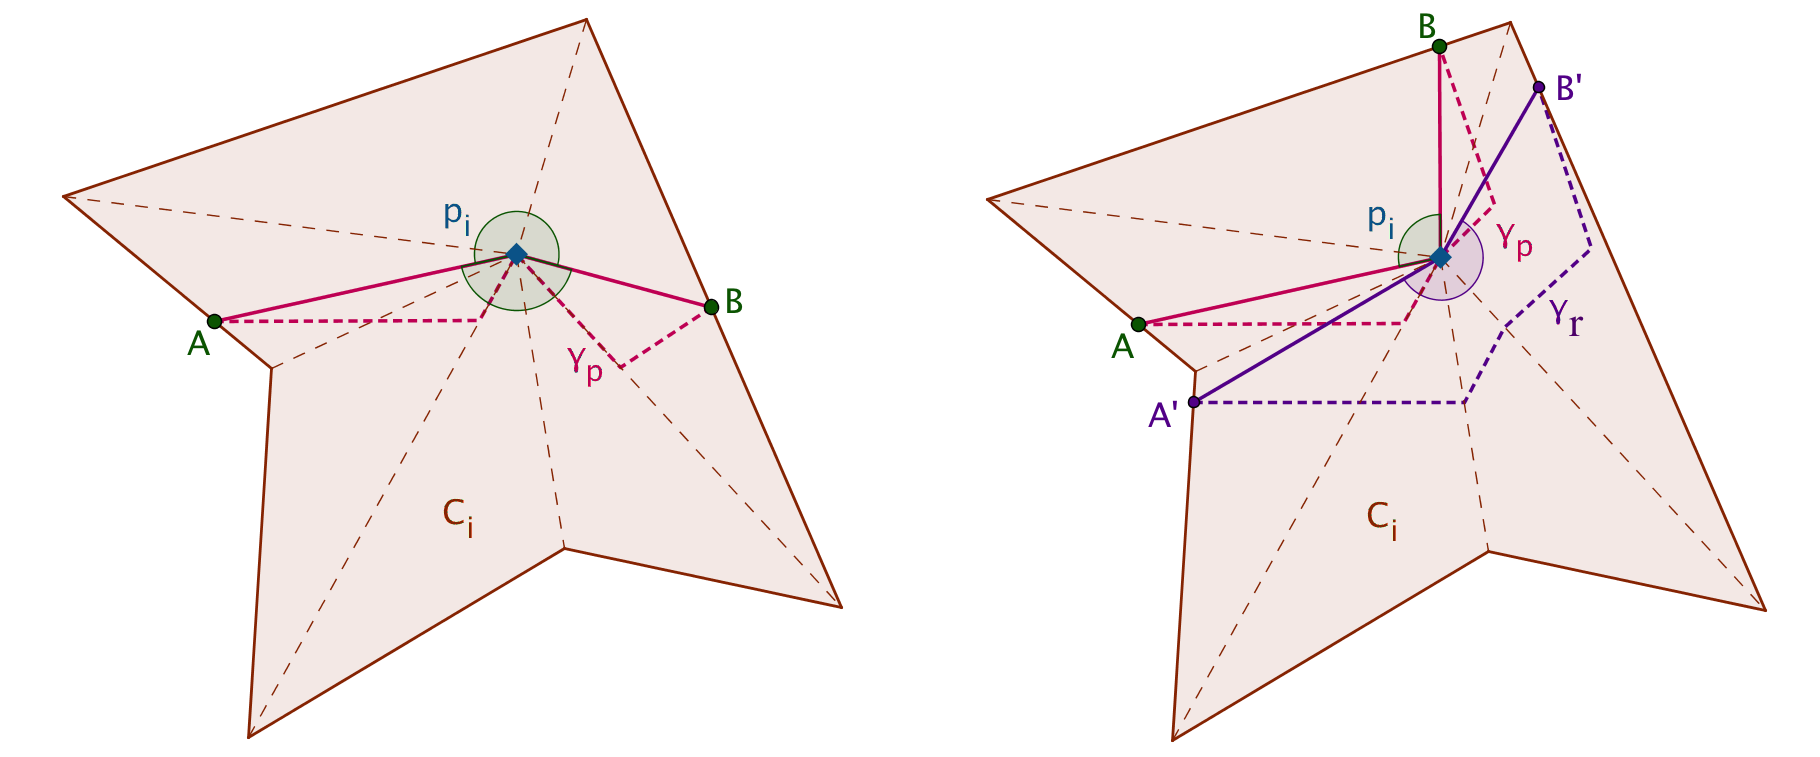
\includegraphics[scale=0.23]{chapeau-1et2}  
		\end{center}
\end{figure}
\item{If the angle formed by $Ap_iB$ on the side of $\mathcal{C}_i^l$ (resp. $\mathcal{C}_i^r$) is $>\pi$ (necessarily, the other will be $<\pi$), we are looking for a fiber $\gamma_l$ (resp. $\gamma_r)$ which can be straightened in $\mathcal{C}_i^l$ (resp. $\mathcal{C}_i^r$) passing through $p_i$, to form an angle equal to $\pi$: it realizes on this side of $Ap_iB$ a shorter path. Therefore, we straighten all the fibers of $\mathcal{C}_i$ on either side of $\gamma_l$ (resp. $\gamma_r)$, as before.}
\tab

\textbf{Case 2 -} We treat the case where no fiber $\beta(t,.)$ is included in $\mathcal{C}_i$, no beak crosses $\mathcal{C}_i$, with $\mathcal{C}_i$ concave.
We test one of the fibers passing through $p_i$, by taking the previous notations.
%\begin{itemize}
%\item{If the two angles formed by $Ap_iB$ are $\geq \pi$, then $\gamma_p$ is straightened out $Ap_iB$, via a decreasing homotopy for the length. Therefore and in the same homotopy ballet, all the other fibers of $\mathcal{C}_i$ can be straightened on a shorter path in $\mathcal{C}_i$, on the side of $Ap_iB$ where they take roots, namely $\mathcal{C}_i^l$ or $\mathcal{C}_i^r$. Remember that no fiber up to now has been cut transversely. Note: a hat is not necessarily convex -- it is at least starred --, then the shortest path between two point of its boundary can come to rest against it.}

%\begin{figure}[h!]
%		\begin{center}
%			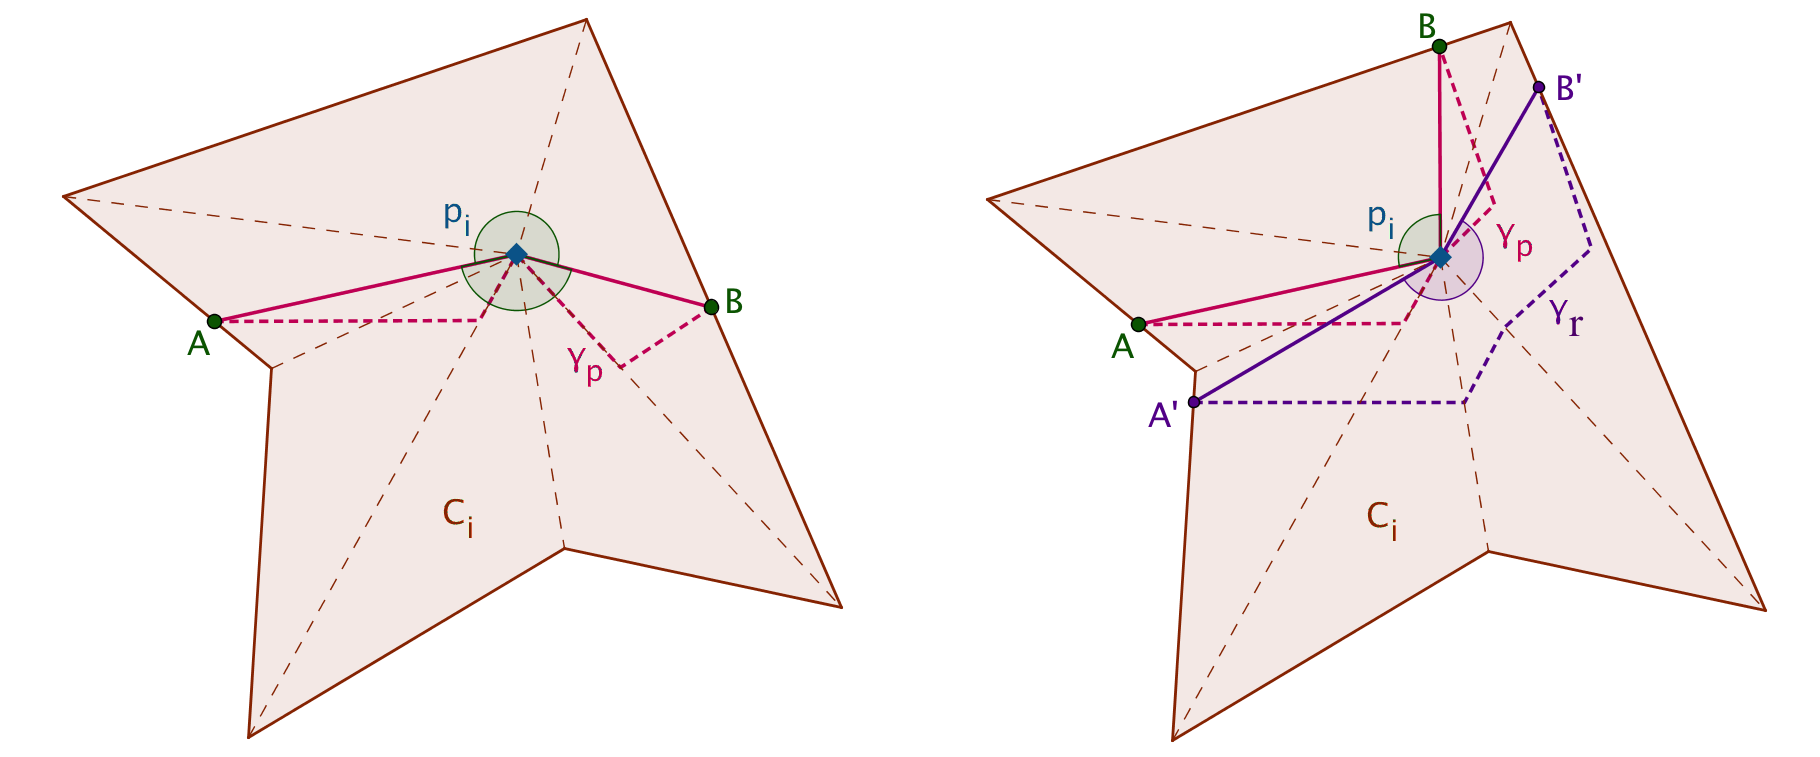
\includegraphics[scale=0.23]{chapeau-1et2}  
%		\end{center}
%\end{figure}
%\item{If the angle formed by $Ap_iB$ on the side of $\mathcal{C}_i^l$ (resp. $\mathcal{C}_i^r$) is $>\pi$ (necessarily, the other will be $<\pi$), we are looking for a fiber $\gamma_l$ (resp. $\gamma_r)$ which can be straightened in $\mathcal{C}_i^l$ (resp. $\mathcal{C}_i^r$) passing through $p_i$, to form an angle equal to $\pi$: it realizes on this side of $Ap_iB$ a shorter path. Therefore, we straighten all the fibers of $\mathcal{C}_i$ on either side of $\gamma_l$ (resp. $\gamma_r)$, as before.}

\end{itemize}
Attention, the presence of a beak, in this district of $\mathcal{C}_i$ can compromise the existence of such a fiber.
\end{proof}


\begin{theorem}[Theorem 2]
There is an algorithm making it possible to construct such a quasi-geodesic.
\end{theorem}
\begin{proof}[Proof of Theorem 2]
Let $\mathcal{E}=\{p_1,\dots,p_n,a_1,\dots,a_m\}$ be the set of vertices and open edges of $S$. To a closed curve $c:I\longrightarrow P$, we associate the word $\mathcal{E}(c)$ whose successive letters (grouped under a bar) are those which designate the elements of $\mathcal{E}$ met by $c(t)$ when $t$ travels $S^1$. We want to give a bound $\eta$ on the combinatorial of $\gamma$, that is to say a bound on the length of $\mathcal{E}(\gamma)$. To each edge $a_{ij}$, we associate a meeting coefficient $k(a_{ij})$ measured as follows:

$$k(a_{ij})=\underset {\begin{matrix}A\in a_{ij}\\B\in \partial(\mathcal{C}_i\cup\mathcal{C}_j)\end{matrix}}{max}\frac{\#([AB], \mathcal{E})-1}{L(AB)}$$
Where $[AB]$ is the shortest way on $S$ beetwen $A$ and $B$ and $\#([AB], \mathcal{E})$ denotes the number of elements of $\mathcal{E}$ met by $[AB]$, transversely or longitudinally if it is an edge.%Notons que $[AB]$ est une quasi-g�od�sique qui ne passe par aucun sommet, si ce n'est �ventuellement en $A$ ou $B$. En effet, le plus court chemin entre deux points qui ne sont pas des sommets �vite toujours ces derniers. Ainsi, il existe un patron local de $P$ sur lequel $[AB]$ est d�velopp� en segment.  \\

\begin{figure}[h!]
		\begin{center}
			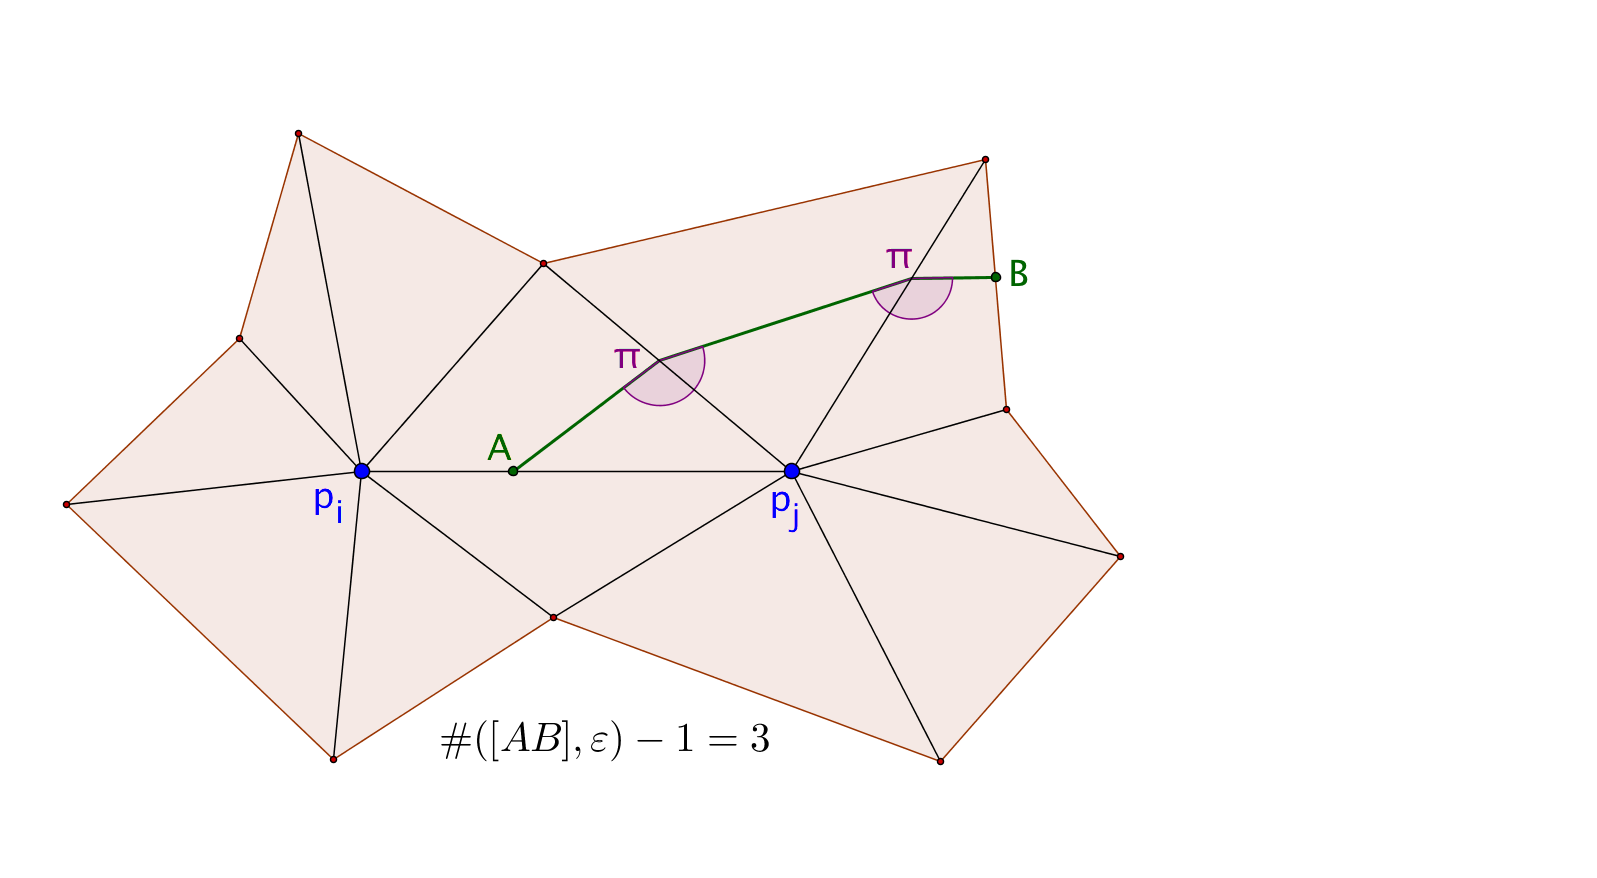
\includegraphics[scale=0.9]{double-chapeau}  
		\end{center}
\end{figure}

{\setlength{\parindent}{0pt}We then have an expression of $\eta$ :}

$$\eta=\left\lceil M\;.\;\underset{a_{ij}}{max}\;k(a_{ij}) \right\rceil$$


\tab


{\setlength{\parindent}{0pt}We consider the set\footnote{Of cardinal $n(n+m)^{\eta-1}$} of $(\eta+1)$-letter words written in the alphabet $\mathcal{E}$, beginning and ending with the same vertex name, noted $p_{\star}$. A \textit{valid} word must contain only three types of sequences :}
\begin{itemize}
\item{An edge crimped by its two ends.}
\item{An edge crimped by the two opposite vertices of the triangles joined at this edge.}
\item{A series of adjacent two by two edges (except triplets $a_{ij}a_{jk}a_{ij}$ and $a_{ij}a_{jk}a_{ki}$), preceded by the vertex opposite the first edge (but not attached to the second) and followed by the vertex opposite last edge (but not attached to the penultimate).\\}
\end{itemize}
To $\gamma$ necessarily corresponds such a word, noted $\mathcal{E}(\gamma)$. Conversely, to a word $x=\overline{p_{\star}l_1\dots l_{\eta-1}p_{\star}}$ corresponds a simple and closed quasi-geodesic if it satisfies, from left to right, the following test :
\begin{itemize}
\item{First case: $\overline{p_ia_{ij}p_j}$ takes place in $x$. We save the path $[p_i,p_j]$ along $a_{ij}$.}
\item{Second case: $\overline{p_ia_{k_1k_2}p_j}$ takes place in $x$, where $(p_i,p_{k_1},p_{k_2})$ and $(p_j,p_{k_1},p_{k_2})$ designate two adjacent triangles. We save the path $[p_i,p_j]$ through the flattening of the two triangles in question, unless it is not convex, in which case the test fails.}
\item{Third case: two vertices $p_i$ and $p_j$ surround a sequence $\overline{a_{k_1}\dots a_{k_r}}$ in $x$. We associate with $a_{k_1}$ its two ends noted $p_{s_0},p_{s_1}$ and for $l\geq 2$, we associate with each $a_{k_l}$ the vertex $p_{s_l}$ it does not share with $a_{k_{l-1}}$. Also, we have a decreasing function $f:l\mapsto f(l)$ such that $p_{s_l}$ and $p_{s_{f(l)}}$ are the ends of $a_{k_l}$. We send the vertices $(p_i,p_{s_1},\dots , p_{k_r}p_j)$ in an oriented plane coordinate system, so that all the triangles keep their metric and their relative orientations (we assume that $0<(\overrightarrow{p_ip_{s_0}},\overrightarrow{p_ip_{s_1}})<\pi$).



\begin{figure}[h!]
		\begin{center}
			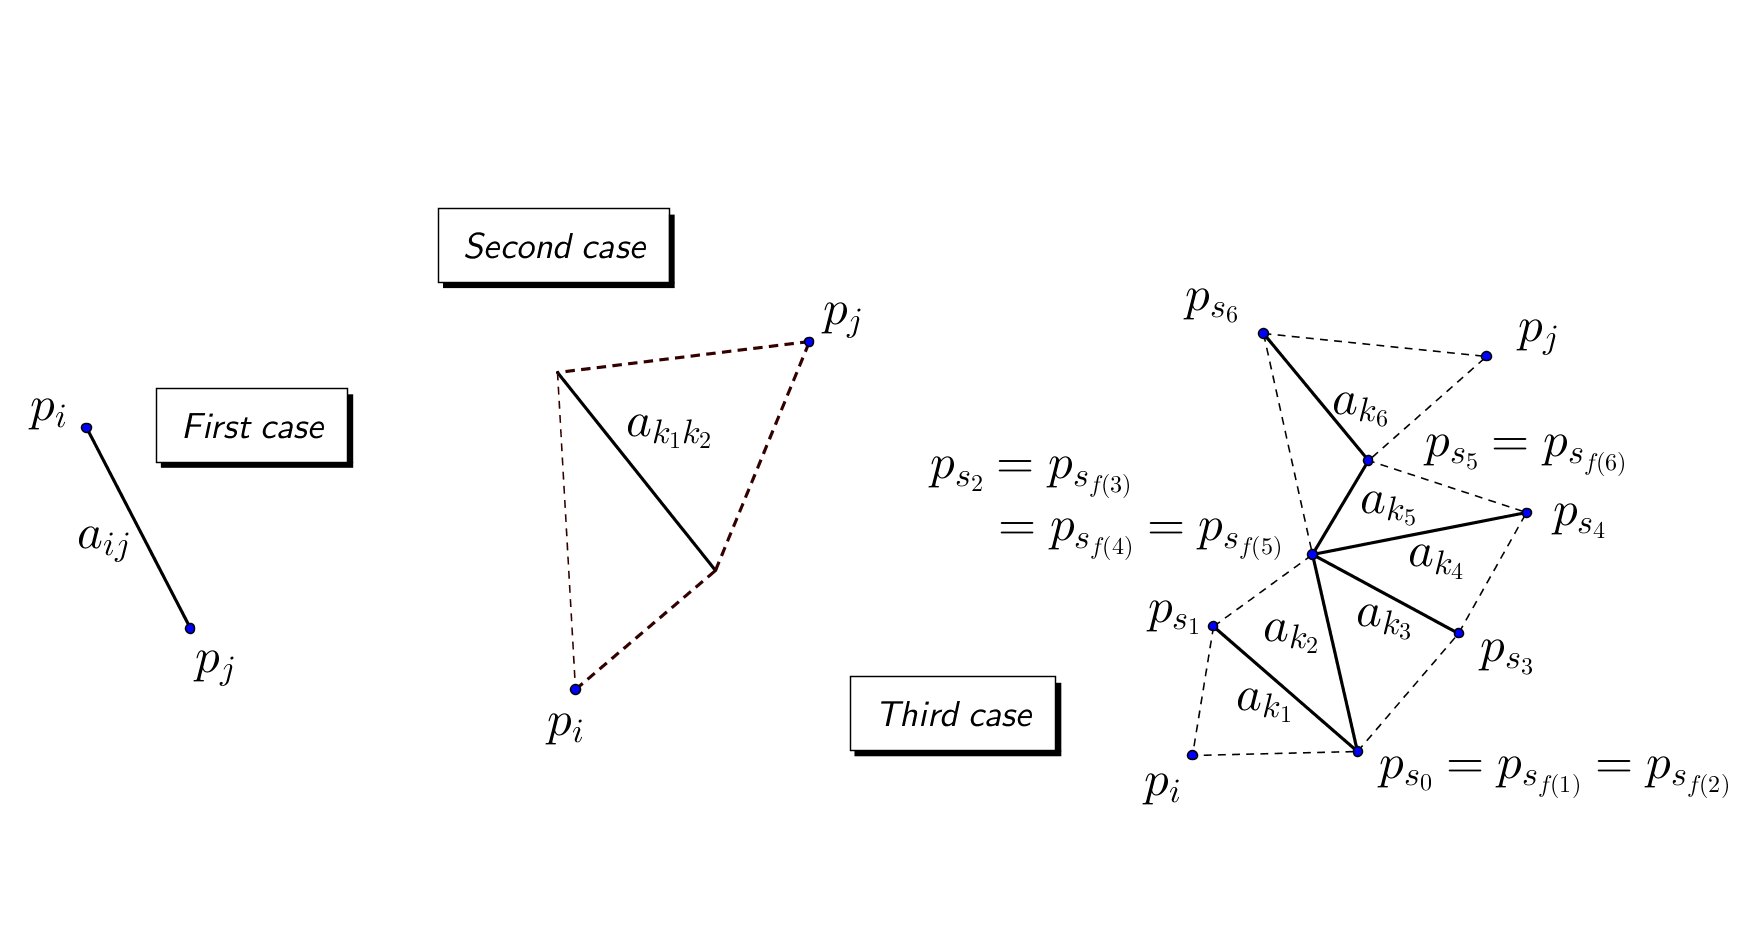
\includegraphics[scale=1.1]{cas-test.png}  
		\end{center}
\end{figure}


We endow ourselves with Boolean functions determining whether a point is located to the left (resp. the right) of an oriented line $(p_i,\overrightarrow{u})$, strictly or not: $p\mapsto (p<u)$, $p\mapsto (p\leq u)$ (resp. $p\mapsto (p>u)$, $p\mapsto (p\geq u)$). The following algorithm evaluates this syllable of $x$:\\ \\
$u=\overrightarrow{p_ip_{k_1}}$\\
$v=\overrightarrow{p_ip_{k_2}}$\\
$\tau=1$\\
For $l$ from $3$ to $r$ and as long as $\tau==1$ :
	\begin{itemize}
	
	
	\item[]{If $(p_{s_l}\leq v)$ with $(p_{s_{f(l)}}\leq v)$: then $\tau=0$.}
	\item[]{If $(p_{s_l}\geq u)$ with $(p_{s_{f(l)}}\geq u)$: then $\tau=0$.}
	\item[]{If $(p_{s_l}< u)$ and $(p_{s_l}> v)$:}
	\begin{itemize}
	\item[]{If $(p_{s_{f(l)}}\geq u)$: then $v=\overrightarrow{p_ip_{s_l}}$}
	\item[]{If $(p_{s_{f(l)}}\leq v)$: then $u=\overrightarrow{p_ip_{s_l}}$}
	\end{itemize}
	\end{itemize}
		
		 
If $(p_j>u)$ or $(p_j<v)$: then 	$\tau=0$.\\	
Only if $\tau==1$, we save the path $[p_i,p_j]$ through this local pattern.\\


} 
\end{itemize}
Finally, we check the angles induced by the paths saved upstream and downstream of each vertex appearing in $x$. If they satisfy the conditions of a quasi-geodesic, we can say that $x$ is the word of a quasi-geodesic.\\


%Dans les trois cas :
%\begin{itemize}

%\item{Si $p_i=p_{\star}$, on continue le test � partir de $p_j$.}
%\item{Si $p_i\neq p_{\star}$, alors des trac�s en aval et en amont de $p_i$ on �t� enregistr�s. Le test est positif si l'angle en $p_i$ form� par ces deux trac�s satisfait aux conditions d'une quasi-g�od�sique.}
%\item{Si $p_j=p_{\star}$, alors des trac�s en aval et en amont de $p_{\star}$ on �t� enregistr�s. Le test est positif si l'angle en $p_{\star}$ form� par ces deux trac�s satisfait aux conditions d'une quasi-g�od�sique.}


\begin{figure}[h!]
		\begin{center}
			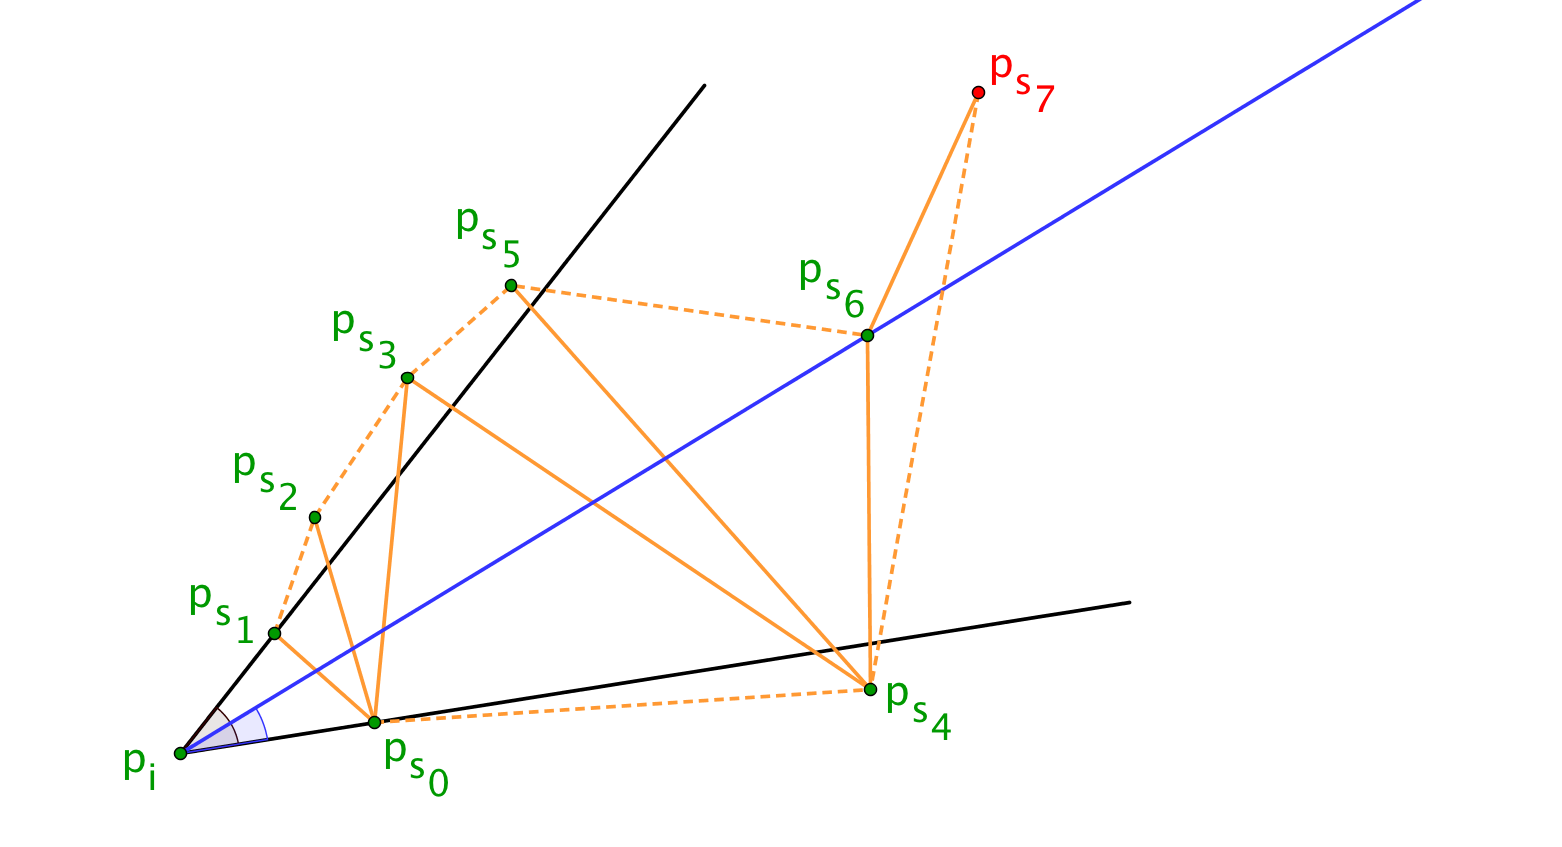
\includegraphics[scale=1]{test-secteur.png}  
		\end{center}
\end{figure}



%mesure les deux angles $(\overrightarrow{p_jp_0},\overrightarrow{p_jp_{k_1}})$ et $(\overrightarrow{p_jp_0},\overrightarrow{p_jp_{k_1}})$ o� $p_{k_1}$ et $p_{k_2}$ sont les sommets voisins de $p_j$ dans $F(p_0,p_j)$.}

%\end{itemize}

{\setlength{\parindent}{0pt}At least one of the valid words must pass the test, starting with $\overline{\gamma}$.\\
Thus, \textbf{the test provides the construction of a quasi-geodesic on $P$}}.
\end{proof}







\end{document}